\section{Modello di sviluppo}
Per lo sviluppo del progetto \textit{Etherless} abbiamo deciso di adottare il \textbf{modello incrementale}.
%aggiungere descrizione
  \subsection{Modello incrementale}
    \begin{figure}[h!]
      \centering
      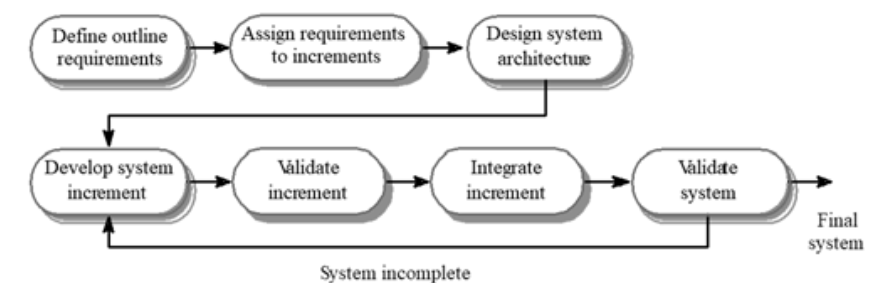
\includegraphics[width=0.9\textwidth]{./res/img/modello_incr.png}
      \caption{Rappresentazione del modello incrementale}
    \end{figure}
    L'adottarsi di un modello di sviluppo incrementale implica lo sviluppo del prodotto tramite multipli rilasci successivi, ognuno dei quali implementa una nuova funzionalità che viene incorporata nel sistema. Questi rilasci sono detti appunto "incrementi". Il numero di incrementi e le funzionalità da implementare all'interno di ognuno sono identificati a partire dai requisiti esposti dal Proponente\ped{\textit{G}} e analizzati dal gruppo \Gruppo{}. Gli incrementi sono ordinati in modo da iniziare con quelli che contengono funzionalità a priorità più alta. All'inizio di ogni incremento si descrivono in dettaglio i requisiti che verranno soddisfatti con il suo completamento, per poi procedere con lo sviluppo. L'incremento viene quindi aggiunto al prodotto e si procede con l'incremento successivo. Per garantire l'efficacia del modello di sviluppo, durante la fase di sviluppo non sono permesse modifiche dei requisiti, a meno che questi non vadano soddisfatti durante incrementi successivi.\\
    Il modello incrementale è stato ritenuto preferibile considerando i seguenti vantaggi:
    \begin{itemize}
      \item ogni incremento porta un valore aggiunto, spingendo verso un'avanzamento continuo del progetto;
      \item sviluppo delle funzionalità più importanti all'inizio grazie all'ordinamento degli incrementi;
      \item i requisiti più importanti vengono chiariti negli stadi iniziali della realizzazione del prodotto;
      \item l'uso di questo modello di sviluppo favorisce lo sviluppo di prototipi funzionanti, che a loro volta favoriscono la validazione dei requisiti e la comunicazione con il Proponente\ped{\textit{G}}.
    \end{itemize}
